\documentclass[a4paper,10pt]{article}
\usepackage[utf8]{inputenc}
\usepackage{graphicx}
\usepackage{xcolor}
\usepackage{listings}
\graphicspath{ {./graphs/} }
\graphicspath{ {./code/} }

\definecolor{mGreen}{rgb}{0,0.6,0}
\definecolor{mGray}{rgb}{0.5,0.5,0.5}
\definecolor{mPurple}{rgb}{0.58,0,0.82}
\definecolor{backgroundColour}{rgb}{0.95,0.95,0.92}

\lstdefinestyle{CStyle}{
    backgroundcolor=\color{backgroundColour},   
    commentstyle=\color{mGreen},
    keywordstyle=\color{magenta},
    numberstyle=\tiny\color{mGray},
    stringstyle=\color{mPurple},
    basicstyle=\footnotesize,
    breakatwhitespace=false,         
    breaklines=true,                 
    captionpos=b,                    
    keepspaces=true,                 
    numbers=left,                    
    numbersep=5pt,                  
    showspaces=false,                
    showstringspaces=false,
    showtabs=false,                  
    tabsize=2,
    language=C
}


\title{\textbf{Operativsystem ID1206} \\ 
\textbf{Malloc \& Free}}

\author{Axel Karlsson}

\begin{document}

\maketitle
\textbf
{\\\\1. Inledning\\\\}
Denna rapport är skriven i syfte av att redovisa mitt arbete med seminarieuppgift två, malloc \& free, i kursen ID1206 Operativsystem. Den givna uppgiften var att implementera en egen version av C funktionera malloc och free (hänvisas framöver till som "malloc"), vars funktion är att hantera dynamisk minnesallokering i ett C program. I den första delen av rapporten redovisar jag min implementation av dalloc och malloc enligt uppgiftsbeskivningen, och i den andra delen går jag igenom den förbättring jag valde att göra.

\maketitle
\textbf
{\\\\1.2 Varför malloc?\\\\}
Malloc är en del av standardbiblioteket i C (stdlib), och är ett verktyg vi kan använda för att kunna allokera minne vid runtime i ett C program. Vi skulle kunna få mina med hjälp av ett systemanrop, till exempel sbrk() eller mmap(), men då dessa anrop är både tids-och prestandakrävande använder vi malloc. Det vi vill uppnå med malloc är att minska antalet systemanrop vi behöver göra genom att göra ett systemanrop och reservera en stor mängd minna, som vi sedan delar ut inom processen med malloc.

\maketitle
\textbf
{\\\\2. Problembeskrivning \& lösningar\\\\}
Det svåraste problemet att lösa i en malloc-liknande funktion är att hantera minne som frigörs på ett sådant sätt att det inte fragmenteras i allt för stor grad. Det finns en uppsjö av strategier för att lösa detta problem, och några av dem har jag implementerat i min malloc funktion.

\maketitle
\textbf
{\\\\2.1 Den givna implementationen av dalloc \& dfree\\\\}
Den implementation av malloc som var given i uppgiftens instruktioner är byggd omkring två datastrukturer, en länkad lista kallad freelist och en struct kallad head. Vi kombinerar dessa och skapar block av minne, som vi sedan delar ut med api:n dalloc() och dfree(). Dessa block lagras i ett datasegment som vi har reserverat i minnet med mmap(). 


\maketitle
\textbf
{\\\\2.2 Möjliga förbättringar\\\\}
I uppgiften var det även givet ett antal förslag på förbättringar på dalloc var av vi skulle implementera åtminstonne en. Jag har valt att implementera möjligheten att skapa fler arenor, vilket möjliggör en större heap samt fler möjligheter för multitrådad programmering.  Min implementation bygger på datastrukturen arena, som har samma funktionalitet som arenan i den givan implementationen. Dessa structs lagras i en länkad lista som kan utökas vid behov. Structen arena innehåller 3 pekare; arena, flist och next. Arena och flist fungerar som de globala head structsen med samma namn i den tidigare implementationen. Structen head har nu även en pekare home, som visar vilken arena det blocket ska lagras i när det frigörs.
\begin{lstlisting}[style=CStyle]
  /* En lankad lista av arena structs */
  struct arena {
    struct head* arena;
    struct head* flist;
    struct arena* next;
  };
  struct arena* arena_head = new_arena(); // new_arena() lankar in en ny arena i listan

  ...

  void new_arena() {
    ...
    struct arena new_arena = mmap(24, ...);
    new_arena->arena = mmap(64KB,...);
    new_arena->flist = new_arena->arena;
    ...
    }

\end{lstlisting}
 

\maketitle
\textbf
{\\\\3 Benchmark\\\\}
Min implementation av malloc har benchmarkats med hjälp av ett program benchmark.c. Detta program har4 parametrar: minsize, maxsize, rounds och maxblocks. Programmet innehåller en loop som körs tills vi har kallat dalloc() rounds antal gånger. I varje iteration av loopen kommer antingen dalloc() kallas och efterfråga ett slumpmässigt antal byte mellan min-och maxsize, eller så kallas dfree() på en slumpmässig tidigare allokering. Maxblocks avser det högsta antalet allokeringar som kan existera samtidigt. \\\\
Detta benchmark har körts med alla tre versioner av malloc jag har implementerat (utan merge, med merge och med flera arenor) med följande parameterar:
\begin{itemize}
  \item minsize = 8 bytes
  \item maxsize = 180 bytes
  \item rounds = 5000 rounds
  \item maxblocks = 1000 blocks
\end{itemize}

\maketitle
\textbf
    {\\\\3.1 Resultat\\\\}
    I figur 1 ser vi att versionen av malloc som kan skapa nya arenor har avsevärt störra block än de andra två versionerna. Observera även de upprepade topparna då nya arenor skapas. 
    \begin{figure}[htp]
    \centering
    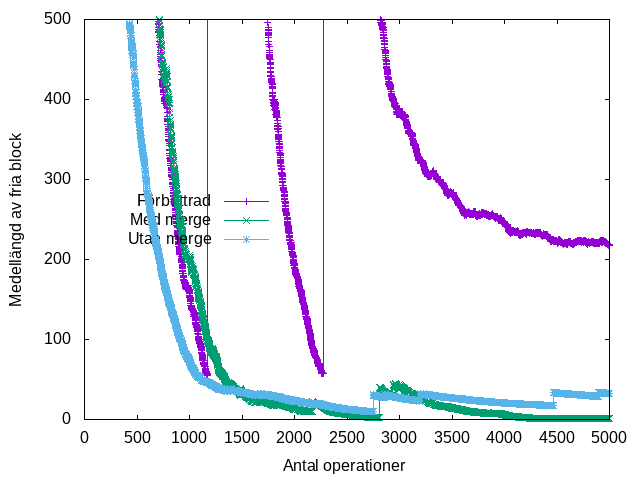
\includegraphics[width=8cm]{benchmark_opsize/all3_sizeops_zoom.png}
    \caption{Genomsnittliga storleken på ett block per dalloc anrop.}
    \label{fig:Graph}
    \end{figure}
    
    
    \begin{figure}[htp]
    \centering
    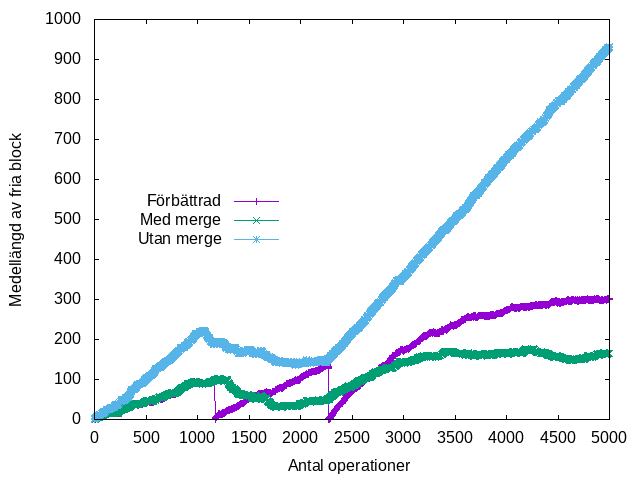
\includegraphics[width=8cm]{benchmark_opsize/all3_lenops.png}
    \caption{Antal fria block per dalloc anrop.}
    \label{fig:Graph}
    \end{figure}
        I figur 2 ser vi att versionen utan merge() får fler fria block ju fler anrop vi gör, samtidigt som de andra versionerna verkar öka långsammare eller avtar. Vi kan även här observera toppar i den lila kurvan då nya arenor skapas

    
\maketitle
\textbf
    {\\\\3.2 Slutsats\\\\}
    Det kan vara svårt att tyda figur 1, men jag behövde begränsa den längs y-axeln då den kommer upp i 64000 när vi har gjort 0 operationer (medellängden på blocken är väldigt stor i början). Det går enkelt att se att den versionen av malloc med förmågan att skapa flera arenor överlag har större fria block än de andra två. Jag vet inte riktigt hur jag ska tolka detta resultat, men jag misstänker att vi tillslut skulle få en medellängd närmre de andra om vi körde benchmarket tillräckligt länge då den i teorin borde vara samma som versionen med merge. \\\\

I figur två ser vi att versionen utan merge har avsevärt många fler fria block än de andra två. Min första instinkt sade mig att detta kan tolkas som att den har fler små block medans de andra två har få stora, men med tanke på resultaten i figur 1 vet jag inte om det är en korrekt tolkning.

\maketitle
\textbf
    {\\\\Reflektion\\\\}
    Resultaten jag fick var oväntade, särskilt att den genomsnittliga blockstorleken (figur 1) var så pass lika för alla tre implementationer. Jag misstänker att detta beror på min testmetod, då versionen av malloc med merge och utan flera arenar i princip är given i uppgiftens instruktioner, och därför förutsätter jag att den är någolunda optimerad. Förutom en mer rafinerad testmetod finns det flera förslag till förbättringar som jag inte har försökt mig på, som möjligtvis skulle kunna ge oss en ännu bättre dalloc. 

\end{document}
